\documentclass{article}
\usepackage[T1]{fontenc}
\usepackage[utf8]{inputenc}
\usepackage[spanish]{babel}
\usepackage{amssymb, amsmath, amsbsy} % simbolitos
\usepackage{multirow} % para tablas
\usepackage{enumerate}
\usepackage{graphicx}

\title{Programa 1 - Adoquinamiento\\ Análisis de algoritmos}
\author{Peto Gutiérrez Emmanuel \\ María de Luz Gasca Soto}
\begin {document}
\maketitle

\section{Introducción}

El problema del adoquinamiento consiste en pavimentar una región dividida en cuadrados iguales.
La región tiene un área de $m \times m$ cuadrados. A partir del cuadrado especial (el cual se coloca
arbitrariamente en el área), se pavimenta con el adoquín formado por tres cuadrados en forma de {\sf L}.

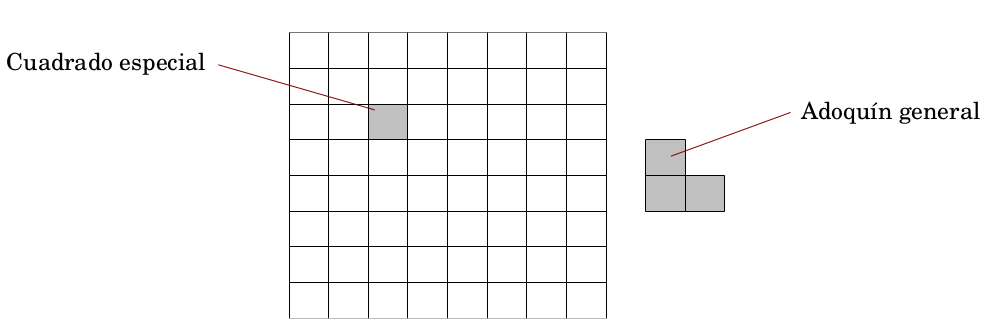
\includegraphics[scale=0.4]{ejemplo1}

\section{Planteamiento del problema}
Sea $m$ una potencia de 2, adoquinar la región de $m \times m$ con el adoquín dado, cubriendo cada cuadrado
exactamente una vez, con excepción del cuadrado especial, el cual no será cubierto por ningún
adoquín.

\section{Implementación}
Se debe hacer un programa en Java para resolver el problema. Pueden usar una interfaz gráfica para mostrar el resultado.

El problema se puede ver como colorear un tablero con {\sf L}'s, de tal forma que 3 cuadros con el mismo color  son adyacentes formando la {\sf L}, pero estos no pueden ser adyacentes a otra {\sf L} con el mismo color.

El siguiente ejemplo muestra una coloración con el \textit{cuadro especial} en (13,6) y $m = 2^4 = 16$:

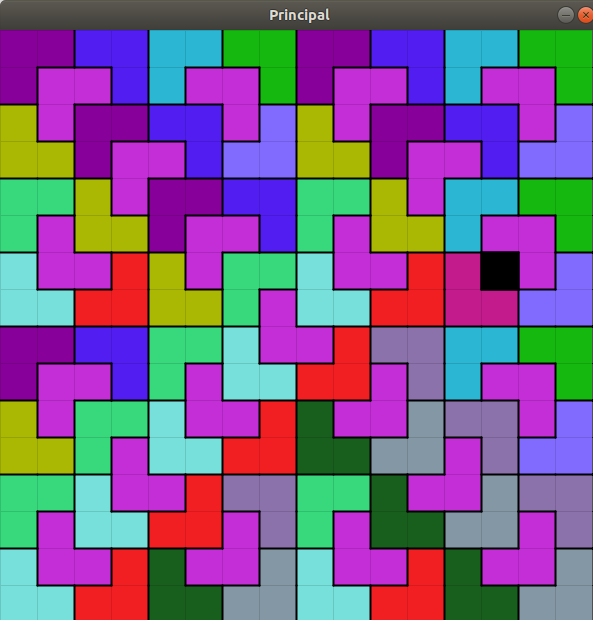
\includegraphics[scale=0.4]{ejemplo2}

Aquí el mismo ejemplo pero sin colores:

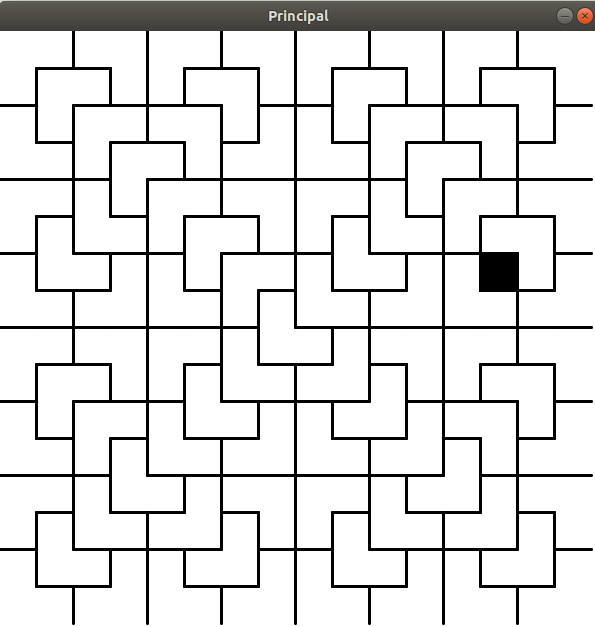
\includegraphics[scale=0.4]{ejemplo3}

Esto se hizo usando \textit{core.jar} de Processing, pero lo pueden hacer con cualquier herramienta.

Un color se puede representar como un número o una letra en una matriz. Si no hacen interfaz, deben imprimir la matriz resultante.\\

La matriz relacionada al ejemplo anterior es la siguiente(en mi implementación):

\begin{table}[h]
\begin{center}
\begin{tabular}{|l|l|l|l|l|l|l|l|l|l|l|l|l|l|l|l|}
\hline
12&12&13&13&11&11&9&9&12&12&13&13&11&11&9&9\\ \hline
12&2&2&13&11&2&2&9&12&2&2&13&11&2&2&9\\ \hline
14&2&12&12&13&13&2&10&14&2&12&12&13&13&2&10\\ \hline
14&14&12&2&2&13&10&10&14&14&12&2&2&13&10&10\\ \hline
8&8&14&2&12&12&13&13&8&8&14&2&11&11&9&9\\ \hline
8&2&14&14&12&2&2&13&8&2&14&14&11&2&2&9\\ \hline
7&2&2&6&14&2&8&8&7&2&2&6&1&0&2&10\\ \hline
7&7&6&6&14&14&8&2&7&7&6&6&1&1&10&10\\ \hline
12&12&13&13&8&8&7&2&2&6&3&3&11&11&9&9\\ \hline
12&2&2&13&8&2&7&7&6&6&2&3&11&2&2&9\\ \hline
14&2&8&8&7&2&2&6&5&2&2&4&3&3&2&10\\ \hline
14&14&8&2&7&7&6&6&5&5&4&4&2&3&10&10 \\ \hline
8&8&7&2&2&6&3&3&8&8&5&2&2&4&3&3\\ \hline
8&2&7&7&6&6&2&3&8&2&5&5&4&4&2&3\\ \hline
7&2&2&6&5&2&2&4&7&2&2&6&5&2&2&4\\ \hline
7&7&6&6&5&5&4&4&7&7&6&6&5&5&4&4\\ \hline
\end{tabular}
\end{center}
\end{table}

\newpage

\section{Detalles}

\begin{itemize}
\item Se puede hacer iterativo o recursivo. Son libres de usar cualquier implementación.
\item Este programa se entrega de forma individual.
\item Si su carpeta contiene un ejecutable(como *.jar) enviarlo como un enlace de dropbox o drive.
\item El problema viene explicado en las notas de clase, Sección 3.3.4 pp. 45-46.
\end{itemize}

\section{Entrega}
\begin{itemize}
\item Deben entregarlo como un archivo comprimido de una carpeta con el mismo nombre.
\item La carpeta debe ser: \textbf{Programa1\_ApellidopaternoApellidomaterno}. Por ejemplo \textbf{Programa1\_PetoGutierrez}.
\item Su carpeta debe contener un archivo \textit{readme} que contenga: número de cuenta, nombre completo, correo y las instrucciones para compilar y ejecutar su programa.
\item El asunto debe ser: \textbf{[AAlgoritmos]ProgramaN}, o sea, [AAlgoritmos]Programa1 en este caso.
\end{itemize}

\end {document}